\capitulo{FUNDAMENTAÇÃO TEÓRICA}
\label{sec:fundamentacao}

Este capítulo tem como princípio apresentar os principais conceitos chave para a compreensão deste trabalho. Os conceitos que serão apresentados são, \textbf{Evasão na Educação a Distância}, \textbf{Mineração de Dados Educacionais}, \textbf{Extração de Conhecimento} e \textbf{Sistemas Multiagente}. Os conceitos destacados são os elementos mais importantes que proporcionam a base para o desenvolvimento deste trabalho.

\secao{Evasão na Educação a Distância}
\label{sec:evasao}

A Educação a Distância (EAD) é o nome atribuído a uma modalidade de ensino que tem como característica principal o ensino e aprendizagem em que alunos e professores não necessitam estar juntos em um ambiente físico como uma sala de aula durante a maior parte do tempo do curso \cite{cambruzzi2014gvwise}. A interação entre docentes e discentes acontece através de Ambientes Virtuais de Aprendizagem (AVA), o \textit{Moodle} é um exemplo de AVA, onde professores, tutores e alunos podem interagir entre si. Dependendo das políticas e normas de ensino da instituição, alguns encontros presenciais podem acontecer periodicamente.

Um dos benefícios proporcionados pela EAD é a capacidade de ampliar oportunidades educativas aos indivíduos, desconsiderando qualquer limitação geográfica ou socioeconômica. Devido a essa capacidade de conseguir levar a educação a usuários de diversos lugares, como também a flexibilidade de horários e compromissos com as atividades dos cursos, a EAD é estimulada tanto por iniciativa privada como pública.

Muitos alunos encontram dificuldades em se adaptarem a EAD, isso acontece por causa do método padrão de ensino presencial. Algumas das dificuldades mais encontradas são a falta de tempo e organização dos horários de estudo, a dificuldade de se adaptar a uma tecnologia nova e uma nova forma de aprendizagem onde o aluno tem que se disciplinar e manter o foco. Devido a essas dificuldades encontradas, nos deparamos com um problema na EAD, que é o elevado índice de evasão dos alunos em relação aos seus cursos \cite{kampff2009mineraccao}.

Podemos entender por Evasão na Educação a Distância o ato do aluno desistir do curso em que esteja devidamente matriculado antes da sua conclusão \cite{cambruzzi2014gvwise}. Dentre os motivos que podem levar ao aluno desistir do curso ou a ter características que podem influencia-lo a ter um mau desempenho no curso, podemos dividi-los em duas categorias: Causas Internas e Causas Externas \cite{kampff2009mineraccao}.

Podemos entender como Causas Internas os fatores que partem do AVA ao aluno, como a falta de adaptação à tecnologia utilizada para a aprendizagem, aluno não ter contato constante com computadores, a falta de compromisso e qualificação dos tutores, a falta de disponibilização de materiais de estudo mais didáticos e em alguns casos, o AVA não segue padrões de usabilidade deixando a desejar a facilidade de interação do usuário com a plataforma.

Como Causas Externas podemos entender como os fatores que partem do aluno com a sua vida pessoal, como a rotina corrida do dia a dia o impedindo de ter um horário reservado para se dedicar aos estudos, problemas financeiros, problemas emocionais e por não praticar a auto-disciplina.

Para uma instituição de ensino é fundamental identificar os alunos e as causas que podem leva-los a evasão e assim encontrar formas de lidar com essa situação, proporcionando um melhor acompanhamento ao aluno durante o seu percurso do início à conclusão do curso.

Em um AVA dados são depositados pelos alunos constantemente. Esses dados podem ser compreendidos como a forma que o aluno se comporta no AVA. E através da Mineração de Dados é possível transforma-los em informações. Entre essas informações é possível identificar características que podem apontar perfis de alunos que possuem mau desempenho, que tendem à evasão, bom desempenho e entre outros.

\secao{Mineração de Dados Educacionais}
\label{sec:mineracao}

Devido ao rápido avanço das tecnologias de coleta e armazenamento de dados, as organizações passaram a acumular uma vasta quantidade de dados \cite{tan2006introduction}. Devido a isso foi possível perceber que através deles poderiam ser obtidas informações úteis através da MD (Mineração de Dados), que é uma tecnologia composta por métodos tradicionais de análise de dados com novos algoritmos sofisticados para processar essa quantidade de dados.

Com o grande acúmulo de dados em Instituições de Ensino, surgiu uma subárea da Mineração de Dados, a Mineração de Dados Educacionais (MDE). Esta é uma área em expansão, tendo como principais enfoques os trabalhos relacionados com aprendizagem supervisionada, que é quando o algoritmo é treinado usando exemplos rotulados como uma entrada onde a saída desejada é conhecida, e aprendizagem não supervisionada, que é quando o algoritmo desconhece as classes que rotulam os dados históricos, sendo necessário o próprio algoritmo encontrar e reconhecer os padrões \cite{cambruzzi2014gvwise}.

Essas duas formas de aprendizagem se dividem em técnicas utilizadas no processo de MD. Algumas delas são:
\begin{enumerate}
\item Aprendizagem Supervisionada
\begin{itemize}
\item Classificação: é utilizada para identificar modelos ou subgrupos de dados classificados de acordo com variáveis previamente definidas.
\item Regressão: é uma atividade utilizada para prever valores de dados de acordo com uma função de mapeamento obtida.
\end{itemize}
\item Aprendizagem Não Supervisionada: 
\begin{itemize}
\item Associação: é a atividade responsável por encontrar grupos de dados que possuem relação características em comum.
\item Clusterização: é utilizado para identificar conjunto de categorias ou agrupamentos que possam descrever o comportamento dos dados selecionados.
\end{itemize}
\end{enumerate}

Para cada técnica existe um conjunto de algoritmos. Em um processo de MD é possível selecionar um ou mais algoritmos que sejam necessários para que seja possível obter o resultado esperado.

Um algoritmo de mineração de dados nada mais é que um conjunto de cálculos e heurísticas que a partir de um modelo, eles identificam padrões ou são capazes de predizer valores de atributos. Para que seja possível criar um modelo, o algoritmo analisa os dados fornecidos, verifica padrões e tendências. A escolha do algoritmo adequado não é fácil, pois é necessário analisar o problema do domínio em questão, o conjunto de dados e seus respectivos tipos, o tamanho da base de dados, e entre outros fatores.

Tão importante como definir o modelo de dados encontrado através da MD, é a sua análise e validação. No caso do presente trabalho, que tem como finalidade utilizar predição, foi utilizada a técnica de \textit{cross-validation} através do método \textit{k-fold}. Essa técnica tem como finalidade dividir o conjunto total de dados em $k$ conjuntos iguais. Após o processo de particionamento, um subconjunto é utilizado para teste, os demais $k$-1 subconjuntos são utilizados para estimar os parâmetros e calcular a acurácia do modelo. Esse método irá repetir $k$ vezes esse processo, alternando circularmente o subconjunto de testes \cite{han2011data}. A figura \ref{fig:kfold} explica visualmente em um exemplo como acontece esse processo.

\begin{figure}[!ht]
\caption{\textit{Cross-Validation (k-fold)}}
\centering
\fbox{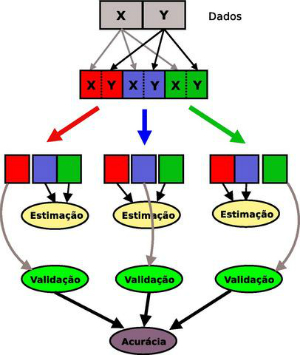
\includegraphics[width=0.62\textwidth]{imagens/kfold.jpg}}
\caption*{Fonte: capturada do Wikipédia}
\label{fig:kfold}
\end{figure}

Para o presente trabalho de acordo com os trabalhos relacionados e pesquisas relacionadas, os algoritmos que mais se adequam para a solução do problema em questão, são algoritmos de classificação, por serem mais eficientes para prever ou descrever conjunto de dados de acordo com categorias nominais (evadido, aprovado, reprovado). Dentre eles os que mais se destacam são:

\begin{enumerate}
\item \textbf{\textit{RuleLearner}}: algoritmo utilizado em técnicas de classificação, que funciona de forma similar ao algoritmo \textit{Repeated Incremental Pruning to Produce Error Reduction} (RIPPER) que é um algoritmo de classificação de eventos que utiliza uma coleção de regras no formato (Se \textbf{\textit{condição}} Então \textbf{\textit{classificação}}), para geração das regras ele tem como critério a \textit{accuracy} (precisão) \cite{cohen1995fast}.
\item \textbf{\textit{ADTree}}: algoritmo de classificação por árvore de decisão, conhecido também como algoritmo de árvore de decisão alternada \cite{freund1999alternating}.
\item \textbf{\textit{SimpleCart}}: é um algoritmo derivado da implementação do algoritmo \textit{Classification and Regression Trees} (CART) que é uma árvore de decisão binária que é construída pela divisão de um nó em dois nós filhos repetidamente. Ela começa com o nó raiz que contém toda a amostra de aprendizagem \cite{breiman1984classification}.
\item \textbf{\textit{J48}}: algoritmo utilizado em técnicas de classificação por  árvore de decisão. Com essa técnica uma árvore de regras é construída para  modelar o processo de classificação. Após a sua criação ela é aplicada a cada  tupla do banco de dados para obter os resultados \cite{quinlan2014c4}.
\item \textbf{\textit{Random Forest}}: é um classificador composto por uma coleção de árvores \{$h_{k}(x)\}, $k = 1,2, \ldots,L, onde $T_{k}$ é um conjunto de amostras aleatórias independentes e identicamente distribuídas, no qual cada árvore vota na classe mais popular para a entrada $x$ \cite{breiman2001random}.
\end{enumerate}

Problemas como evasão de alunos ou mau desempenho em um curso a distância podem ser identificados previamente por técnicas de MD. Gerar esses diagnósticos e identificar os perfis de alunos com essas características é de grande importância para a instituição, pois assim novas formas de resolver esses problemas podem ser desenvolvidas, proporcionando um melhor acompanhamento ao discente.

Tendo como objetivo obter informações úteis à instituição através da MDE, é necessário o desenvolvimento de uma abordagem mais ampla que faça um estudo prévio dos fatores a serem monitorados. Tão importante quanto a seleção dos algoritmos e dos atributos a serem analisados, é a forma que essas informações serão obtidas e de que forma essa analise irá se adaptar periodicamente a quantidade de eventos que podem acontecer.

\secao{Extração de Conhecimento (KDD – Knowledge Discovery in Databases)}
\label{sec:extracao}

Extração do conhecimento ou processo de KDD derivado do inglês \textit{knowledge- discovery in databases}, é um processo que busca identificar potenciais padrões úteis, que estejam embutidos nos dados e, tornando-os compreensíveis para um determinado contexto \cite{fayyad1996knowledge}. A figura \ref{fig:processokdd} demonstra sequencialmente as etapas para descoberta de conhecimento.

\begin{figure}[!ht]
\caption{Processo de KDD}
\centering
\fbox{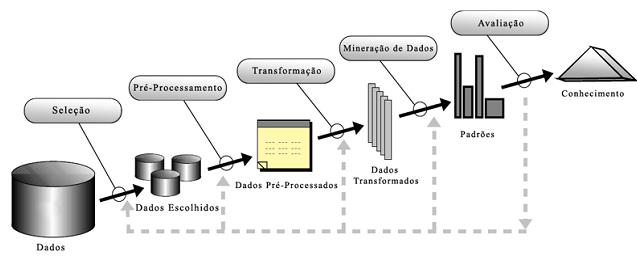
\includegraphics[width=0.75\textwidth]{imagens/kdd.jpg}}
\caption*{Fonte: \cite{fayyad1996knowledge}}
\label{fig:processokdd}
\end{figure}

O processo de KDD consiste em uma sequência de etapas que devem ser executadas sequencialmente, pois ao final de cada etapa, o resultado obtido serve de auxílio para a etapa seguinte, podendo repetir etapas anteriores sempre que necessário. São etapas do processo de KDD: seleção, pré-processamento e limpeza, transformação dos dados, mineração de dados,interpretação e avaliação dos dados. A seguir cada subseção irá explorar sucintamente cada uma das etapas do processo de KDD.

\subsecao{Seleção}

A etapa de Seleção é a primeira no processo de KDD, é a etapa em que serão definidas a (s) fonte (s) que se relacionam com o domínio para a extração dos dados apropriados para o contexto. Ela é trivial para obter êxito no resultado final. Devido as fontes dos dados poderem vir de fontes heterogêneas (planilhas, banco de dados relacional/não relacional, formulários) como também possuírem diversos formatos (CSV, ARFF, TXT), ela se torna uma atividade complexa, assim sendo necessário padroniza-los, integra-los e limpa-los.

\subsecao{Pré-processamento e Limpeza}

Devido os dados estarem possivelmente em formatos diferentes como também terem sido coletados de fontes diferentes, o subconjunto selecionado pode vir com alguns erros, como dados ausentes, dados com erro, registros duplicados e ruídos, tornando-se necessário tratar esses dados por um processo de integração, padronização e limpeza, para que seja gerado um subconjunto de dados que possa representar o domínio.

Ao realizar as operações dessa etapa, apesar de existirem ferramentas que podem auxiliar nesse processo, é de grande importância a presença de um especialista do domínio. Ele é quem mais entende a situação abordada e quem está mais apto a selecionar quais dados são relevantes ou que necessitam ser removidos.

De acordo com Oliveira (\citeyear{oliveira2000processo}) essa etapa de pré-processamento e limpeza
compreende os seguintes aspectos:

\begin{enumerate}
\item \textbf{Padronização dos Valores dos Atributos}: devido ao fato de que os dados possam ser recuperados de várias fontes diferentes, é possível que dados que representam atributos com o mesmo significado possuam tipos diferentes. Por exemplo, o controle de acesso de funcionários em uma determinada base de dados está representada por “DIRETOR”, “SUPERVISOR”, “ATENDENTE”, enquanto em outra base de dados está representado por “1”, “2”, “3”, portanto, é necessário padronizar esses dados para um tipo em comum.
\item \textbf{Remoção de Registros Duplicados}: em determinadas situações após o processo de integração dos dados, podem aparecer registros duplicados ou que representem a mesma informação, porém de forma diferente.
\item \textbf{Tratamento e Eliminação de Ruídos}: durante o processo de coleta dos dados desejados é possível que alguns valores possam conter ruídos devido a alguma falha no processo de coleta, por exemplo, tipos de dados não suportados pelo SGBD. Os dados com ruídos em seus valores devem ser corrigidos atribuindo a eles os seus valores corretos ou eliminado-os de acordo com a relevância do mesmo para o processo de KDD.
\item \textbf{Tratamento de Valores Ausentes}: encontrar campos em tabelas de banco de dados nulos ou formulários com campos ignorados e não preenchidos é tão comum quanto encontrar dados com valores duplicados. Para solucionar esse problema é preciso estabelecer regras e critérios para correção para decidir se esses dados irão ser ignorados, preenchidos com o valor correspondente ou algum padrão para valoração de campos nulos, e sempre procurando resolver com o método mais adequado que influencia positivamente para o processo de KDD.
\end{enumerate}

Após a realização dessa etapa, os dados já estarão selecionados, pré-processados e limpos, porém ainda não foram formatados adequadamente para que os algoritmos da etapa de MD sejam aplicados.

\subsecao{Transformação dos Dados}

Esta etapa é crucial para que os algoritmos que serão aplicados na etapa de MD consigam obter êxito em seus objetivos com eficiência e eficácia, portanto, faz-se necessário realizar a formatação e o armazenamento adequado dos dados.

Durante esta etapa é possível obter valores através de outros dados, denominando-os de valores derivados. Por exemplo o lucro mensal de uma empresa que poderá ser obtido através da somatória das transações efetuadas durante o mês desejado.

\subsecao{Mineração dos Dados}

Esta etapa é a mais importante de todo o processo de KDD, pois é nela onde as informações relevantes são obtidas.

De acordo Tan (\citeyear{tan2006introduction}), MD é uma forma de explorar e analisar dados de forma supervisionada ou não supervisionada, com o intuito de perceber regras e padrões em grandes fontes de dados afim de obter informações relevantes para algum objetivo ou entidade. Mais detalhes sobre MD já foram descritos na Seção \ref{sec:mineracao}.

\subsecao{Interpretação e Avaliação}

Através dessa etapa é possível chegar à informação desejada, através da interpretação e avaliação dos padrões encontrados através da etapa de MD. Os usuários podem utilizar diversas ferramentas com funcionalidades estatísticas e de visualização para validarem ou julgarem um padrão irrelevante.

Ao finalizar essa etapa, caso não sejam encontradas informações relevantes ou informações esperadas, é preciso retornar aos passos anteriores para corrigir os possíveis problemas até encontrar as informações necessárias.

De acordo com a literatura da área, existem várias ferramentas que podem auxiliar durante o processo de KDD. Dentre elas é possível citar o RapidMiner\footnote{Disponível em: https://rapidminer.com}, Weka\footnote{Disponível em: http://www.cs.waikato.ac.nz/ml/weka} e o Elki\footnote{Disponível em: http://elki.dbs.ifi.lmu.de}, que são ferramentas de código aberto desenvolvidas em Java.

\secao{Sistemas Multiagentes}
\label{sec:multiagentes}

Sistemas Multiagentes podem ser entendidos como uma subárea da inteligência artificial, composta por agentes que, segundo Russel e Norvig (\citeyear{russel2004inteligencia}), são entidades de software capaz de perceber seu ambiente por meio de sensores e de agir sobre ambientes por intermédio de atuadores, podendo comunicar-se e tendo como princípio conquistar seus objetivos firmados em seus respectivos compromissos.

De acordo com a literatura da área é possível encontrar \textit{frameworks} destinados ao desenvolvimento de SMA’s. Dentre estes é possível destacar a plataforma JADE\footnote{Disponível em: http://jade.tilab.com}(\textit{Java Agent Development Enterprise}). Este \textit{framework} foi desenvolvido na linguagem Java, além de ser um ambiente de execução de agentes, ele simplifica o desenvolvimento de SMA’s através de uma arquitetura que está de acordo com as especificações FIPA\footnote{Disponível em: http://www.fipa.org} (\textit{Foundations of Intelligent Physical Agents}).

A FIPA é uma organização formada para produzir especificações de padrões de software para agentes. Suas especificações consistem em representar um conjunto de normas para promover interação de agentes e os seus serviços. Como exemplo de um possível SMA, será descrita a situação a seguir, dando ênfase aos agentes e à comunicação entre eles.

Em uma determinada cidade existe um corpo de bombeiros, ele possui bombeiros que podem ser entendidos como agentes que possuem o papel de apagar incêndios. Na mesma cidade existem pessoas que como agentes têm o papel de avisar acontecimentos de incêndios. Aqui identificamos dois agentes, o Agente Bombeiro e o Agente Alarmador. Quando acontecer algum incêndio o Agente Alarmador irá enviar uma mensagem para o Agente Bombeiro, por sua vez o Agente Bombeiro irá iniciar os procedimentos para combater o incêndio \cite{batista2008desenvolvendo}.

Nessa situação os dois agentes descritos possuem papéis e características diferentes. Aqui é possível identificar uma aridade binária de acordo com o protocolo de comunicação das especificações FIPA. Uma aridade binaria representa a comunicação de um único emissor com um único receptor. De acordo com as subdivisões dos protocolos de comunicação, também existem casos que os agentes possuem aridade n, isso implica que existe um emissor e vários receptores. De acordo com as especificações FIPA, um protocolo de comunicação entre agentes possui a seguinte estrutura de dados, emissor, receptor (es), linguagem utilizada, funções de codificação e decodificação da linguagem e ações que o receptor deve executar.

-